\documentclass[11pt]{article}
\usepackage[T1]{fontenc}
\usepackage[utf8]{inputenc}
\usepackage[margin=1in]{geometry}
\usepackage{amsmath,booktabs,graphicx,microtype}
\usepackage[section]{placeins}
\usepackage[round,authoryear]{natbib}
\usepackage[colorlinks=true,allcolors=blue]{hyperref}
\setlength{\emergencystretch}{2em}
\title{Do Language Models Have Educational Personalities?\\
Testing Recurring Behavior on New Tutoring Problems}
\author{Anonymous working draft}
\date{}
\begin{document}
\maketitle
\begin{center}
\small\textbf{Incomplete working draft.} Introduction, related work, methods,
archive audit, measurement development, and limitations. Prospective confirmation results,
the empirical abstract, discussion, and conclusion remain to be completed.
\end{center}
\section{Introduction}

Two language models can solve the same exercise correctly while teaching very
differently. One gives the answer and explains it; another asks the student to
complete a step; a third acknowledges the student's frustration before doing
either. Such differences motivate a question about \emph{educational
personality}: do deployed models exhibit recurring teaching tendencies that help
predict how they will respond in a new educational situation?

Answering this question requires more than distinguishing the models' text.
Length, formatting, task instructions, and access to the solution can all produce
recognizable differences. Nor does a model need to behave identically in every
situation to have a recurring tendency. A tutor may consistently explain more
after an erroneous attempt, or acknowledge difficulty specifically when a student
expresses frustration. The empirical question is whether a model's defaults or
its conditional response patterns recur sufficiently to predict new behavior.
An observed difference, a repeatable measurement, and a successful prediction
are distinct steps in that argument.

Education provides concrete choices through which to test this question without
assuming a human personality taxonomy. Revealing a solution and inviting the
student to reason are observable actions; they can co-occur, and neither is
universally the better teaching move. Acknowledging expressed frustration is
also observable without inferring that the model experiences empathy. These
behaviors let us distinguish how a model tends to teach from how accurately it
solves a problem or how much a learner benefits. Our object of study is the
\emph{tutor model's} recurring behavior. It differs from adapting instruction to
an assigned or inferred \emph{student personality}, as in personality-aware
teaching systems \citep{rooein2026pats}.

Prior studies identify model differences through personality-oriented
scenarios and situated behavioral probes \citep{lee2025trait,liu2026bma}.
Educational studies already compare characteristic tutoring-action mixtures
and learn tutor-persona variation from dialogue
\citep{kucheria2025cima,lee2026tutorpersonas}. Building on these observations,
we test the incremental predictive information in deployed models' defaults
and student-state response patterns. The comparison is against the educational
situation, model-specific subject habits, and simple training-output style
profiles, with forecasts locked before new responses are generated.

We organize the investigation around three questions. \textbf{RQ1:} Under the
same educational input, do models show distinguishable defaults that recur
across repeated generations? \textbf{RQ2:} Can those defaults, or model-specific
responses to student state, predict actions on independent source problems?
\textbf{RQ3:} How do the resulting profiles change under neutral rewordings of
the tutor role and explicit teaching instructions? These questions form one
evidence chain. The first establishes recurring differences; the second tests
their predictive value; the third identifies conditions under which they persist
or move.

The study connects an existing educational-output archive to a separate
prospective experiment. The archive contains more than one million raw
prediction records, with different roles, coverage, and repetition histories.
We audit those distinctions before using the archive for exploration. We then
develop observable event measures on a small, permanently excluded pilot and
freeze a source-separated training and confirmation design. Predictions are
fitted and saved before confirmation responses are generated. Model-by-subject
baselines prevent subject-specific habits from being mistaken for student-state
response patterns, while neutral role wording and explicit teaching policies
are manipulated separately on the same inputs.

The resulting claims concern observable tendencies of specified deployments.
They do not establish human-equivalent traits, a latent psychological mechanism,
or learning gains. In particular, a successful default profile does not imply
that a more elaborate conditional profile will improve prediction, and a large
instruction effect does not by itself establish or refute educational
personality. The final conclusions must follow these comparisons, including
measurement failures and limits on transfer.

\section{Related Work}

\paragraph{Personality and situated behavior.}
TRAIT extends personality inventories into scenario-based choices and evaluates
distinctiveness, consistency, and prompting effects \citep{lee2025trait}.
Behavioral Mode Axes uses situated choices across interaction registers,
also evaluates open-ended generations, and studies activation-based control
\citep{liu2026bma}. Separate construction and evaluation scenarios are already
part of that framework. Internal-feature interventions further connect
personality-related representations to behavior across situations
\citep{zhang2026triad}; conversational studies examine contextual variation under
the same assigned personality \citep{han2026contexts}. Together these studies
motivate examining both recurring defaults and conditional expression. Our
deployment-level forecasts test observable educational actions and do not
identify the internal mechanisms responsible for them.

\paragraph{Tutor behavior and educational personas.}
The CIMA comparison studies three LLMs in language-learning dialogues, reporting
characteristic action mixtures and response complexity. Its generation prompt
requests both a response and action labels \citep{kucheria2025cima}. Thus,
describing model-specific teaching styles is an existing research direction.
Tutor-persona steering learns from human tutoring dialogues and evaluates
persona alignment on held-out dialogues \citep{lee2026tutorpersonas}. Our
experiment instead measures the default behavior of multiple deployed
configurations and compares changes caused by controlled student cues and
teaching instructions. We code the visible answers after generation and retain
cross-coder sensitivity; this changes the measurement procedure without
establishing that the resulting labels are ground truth.

\paragraph{Teaching quality and the predictive question.}
MRBench and MathTutorBench organize pedagogical-capability evaluation
\citep{maurya2025mrbench,macina2025mathtutorbench}. PATS studies teaching adapted
to student personality \citep{rooein2026pats}. Our primary target is the
probability of the tutor's next observable behavior under specified conditions.
Predicting that behavior does not rank its educational value. The empirical
addition sought here is a joint account of which default and conditional
profiles predict new-source actions, how those profiles compare with simpler
explanations, and how neutral wording and explicit policies change them on
matched inputs. Source separation and advance prediction locks make these
comparisons auditable; their substantive contribution depends on the resulting
evidence rather than on the procedure alone.

\section{Study Design and Tests}
\label{sec:methods}

We define \emph{educational personality} operationally as recurring defaults
and conditional response patterns that help predict a deployment's behavior on
new educational inputs. The unit is a deployment configuration, including the
requested and returned model names, provider, observation period, and generation
settings. We study MiniMax-M3, MiniMax-M2.7, GLM-5.3, DeepSeek-V4-Pro, and
Doubao-Seed-2.0-Lite. This definition neither assumes human traits nor requires
an invariant ranking across contexts. Figure~\ref{fig:study-design} shows how
the design connects recurrence, prediction, and prompt effects. Complete
materials, measurement rules, estimation details, and protocol history appear
in Appendix~\ref{app:detailed-methods}.

\begin{figure}[t]
\centering
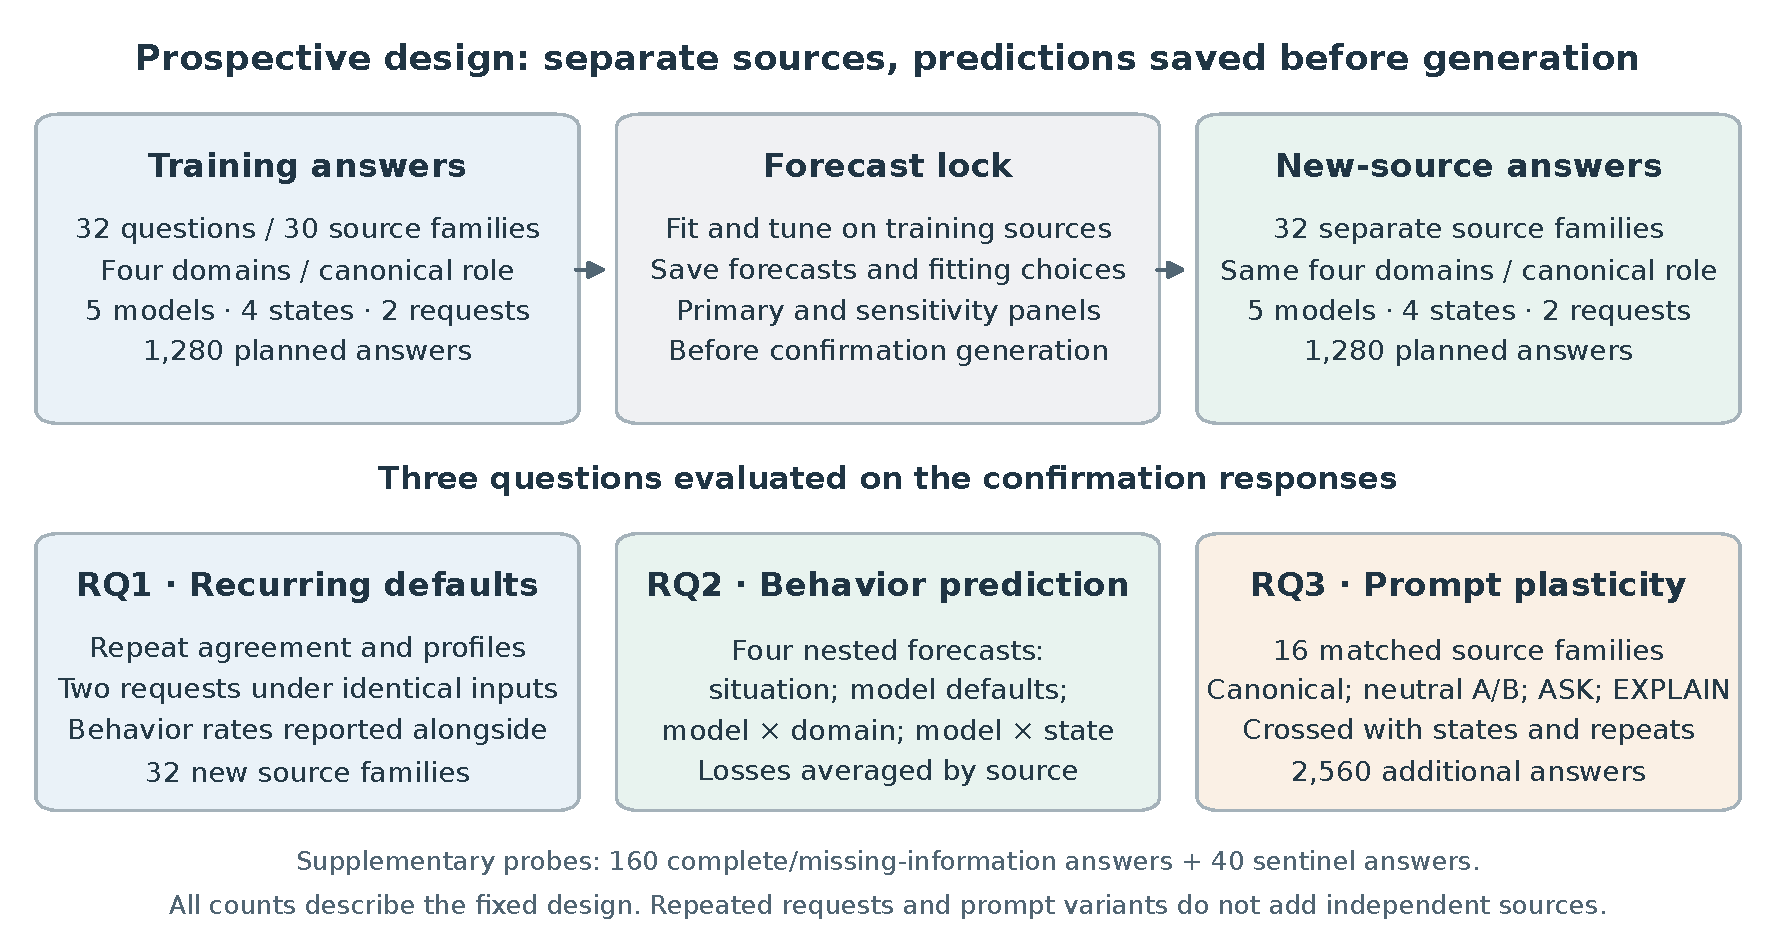
\includegraphics[width=\linewidth]{figures/study_design.pdf}
\caption{Prospective design, with realized response counts. Each main question
crosses five configurations, four student-work/affect conditions, and two
requests. Main training and confirmation source families are separate.
RQ1 and RQ2 use the 32 canonical confirmation sources; RQ3 reuses 16 of them
under additional role arms. Repetitions and prompt variants do not add
independent sources. The four nested forecasts are accompanied by the
training-only style competitor and the sensitivity analyses described below.}
\label{fig:study-design}
\end{figure}

\subsection{Exploration, Measurement Development, and Confirmation}

The million-record archive informed exploration. Its 899,025 successful,
variant-preserving deduplicated records span different roles; 68,799 belong to
nine tutor-response settings under the current-adapter role audit. Historical
prompt and deployment provenance is incomplete (Appendix~A). We therefore keep
archive findings separate from the prospective experiment. An excluded pilot
of 160 answers develops the event measures reported in
Section~\ref{sec:measurement-development}.

The prospective experiment contains 32 training questions in 30 conservative
source families and 32 confirmation questions in 32 separate families. Each
partition has eight questions in mathematics, science, language, and logic/data
reasoning. Related training questions remain grouped during validation, and the
four pilot templates and their numerical substitutions are excluded. Research
agents authored the problems and student messages; two model reviewers checked
all 64 question packages before freezing. The confirmation target is new
sources within these four domains, not unseen domains or representative
classroom interactions.

Each question crosses an erroneous attempt versus correct unfinished work with
an explicitly calm versus frustrated student statement. The work contrast
bundles correctness and progress; the affect contrast manipulates a textual
cue. Every main condition supplies the same instructor reference solution,
marked as unseen by the student. This equalizes solution availability without
eliminating ability or instruction-following differences. Each model--input cell
receives two requests at temperature 0.7 and an 8,192-token output budget.
Training and canonical confirmation each contain 1,280 responses. Additional
prompt arms contribute 2,560 responses on 16 confirmation sources. Secondary
information-opportunity probes and cross-stage sentinels add 160 and 40
responses, respectively, for 5,320 tutor generations. These repetitions
and variants do not add independent sources.

\subsection{Observable Behavior and Recurrence (RQ1)}

The three pilot-selected primary events are \emph{answer revelation}, an
explicit final resolution regardless of correctness; \emph{reasoning
elicitation}, an invitation for the student to perform reasoning that the tutor
has not immediately answered; and \emph{affect acknowledgement}, explicit
recognition of feeling or difficulty beyond generic praise or politeness. These
co-occurring actions are endpoints, not independent latent factors. Five
secondary events remain reported regardless of their results.

MiniMax-M3, DeepSeek-V4-Pro, and GLM-5.3 each code every visible response using
student context, the reference target, and original answer lines. Generator
identity, role arm, repetition, and partition labels are withheld; output style
may still reveal identity. Positive codes require existing nonempty evidence
lines. Primary labels use the majority of three structurally valid codes;
traceability and agreement do not establish semantic ground truth. Repairs
address completion or structure failures, never event labels or disagreement.
One missing training code required a disclosed larger-budget amendment before
prediction locking. Six missing confirmation codes later required a separately
recorded amendment after the original repair limit. Appendix~\ref{app:detailed-methods}
preserves their scope and failures; a supplemental missing-code sensitivity
checks whether the primary conclusions depend on the amended measurements.

RQ1 reports model event rates, state-specific profiles, and positive, negative,
and total agreement across the two requests, with source clustering. Constant
behavior can yield perfect agreement, so recurrence is interpreted alongside
prevalence and predictive value.

\subsection{Locked Prediction on New Sources (RQ2)}

For each event, four nested logistic predictors successively include
subject-by-student-state context, model identity, model-by-subject interactions,
and model-by-student-state interactions. Training-only orthogonalization and
standardization preserve the ridge geometry of earlier feature blocks.
Source-grouped training validation selects the penalty from
$\{0.1,1,10,100\}$; the intercept is unpenalized. All fitted parameters, tuning
choices, and confirmation probabilities are locked before any confirmation
tutor response is generated. No confirmation answer or label enters prediction
fitting. A descriptive style competitor uses only training profiles of log word
count and marked-line fraction.

For each primary event, we test two Brier-loss improvements: adding model
defaults to context, and adding student-state interactions to the
model-by-subject predictor. Losses are averaged within source and equally
across 32 confirmation sources. Six one-sided paired source-level tests use
Holm correction; absolute losses, all gain signs, and source-bootstrap intervals
are reported. Intervals condition on the fitted training profiles and a
source-sampling approximation, not uncertainty over all educational settings
or model families.

\subsection{Prompt Effects and Alternative Explanations (RQ3)}

On 16 sources selected by a frozen hash, each model receives every student state
under the canonical role, two neutral role paraphrases, and explicit ASK and
EXPLAIN instructions. Paired source-level event-rate differences measure both
average displacement and model/state heterogeneity. The neutral equivalence
reference is $\pm0.10$. Nominal multiplicity-adjusted paired-$t$ intervals are
retained, but the additional bounded-source check is too imprecise at sixteen
sources to establish population equivalence. Nonsignificance does not establish
stability. ASK/EXPLAIN effects quantify instruction-driven behavior, not better
teaching. Joint revelation/elicitation rates allow both actions to co-occur
without inferring their order.

Pre-confirmation sensitivity specifications include eight coding panels, five
leave-one-generator analyses, and 200 training-source resamples. Mathematics
and content-error screens evaluate the locked forecasts without refitting;
flagged answers remove the complete five-model comparison slot. Two content
reviewers also receive twelve agent-authored diagnostic controls. These checks
assess dependence on measurement, configurations, training material, and errors;
they do not establish human ground truth or causal control of ability. Their
precise timing, retained coverage rules, and interpretation limits are given in
Appendix~\ref{app:detailed-methods}.

\section{Measurement Development Results}
\label{sec:measurement-development}

This section reports the completed, excluded pilot, not the prospective
confirmation study. Its 160 tutor responses cover only four templates and
therefore do not justify education-wide prevalence or uncertainty estimates.
All responses received three complete event codes after the recorded structural
repairs. Figure~\ref{fig:pilot-measurement} separates agreement on event presence
from agreement on absence, rather than allowing abundant negative examples to
dominate a single agreement statistic.

The three selected primary endpoints have majority-positive counts of 129 for
answer revelation, 61 for reasoning elicitation, and 111 for affect
acknowledgement. Their pairwise positive agreement ranges are 98.04--99.23\%,
89.43--92.19\%, and 97.32--98.63\%, respectively. In contrast, requests for missing
facts have only one majority-positive example: positive agreement ranges from
0--40\% despite high overall agreement. Unsupported ability attribution also
has weaker positive agreement, ranging from 33.33--51.16\%. These results support
different measurement priorities; they do not validate a fixed-dimensional
personality taxonomy.

\begin{figure}[tb]
\centering
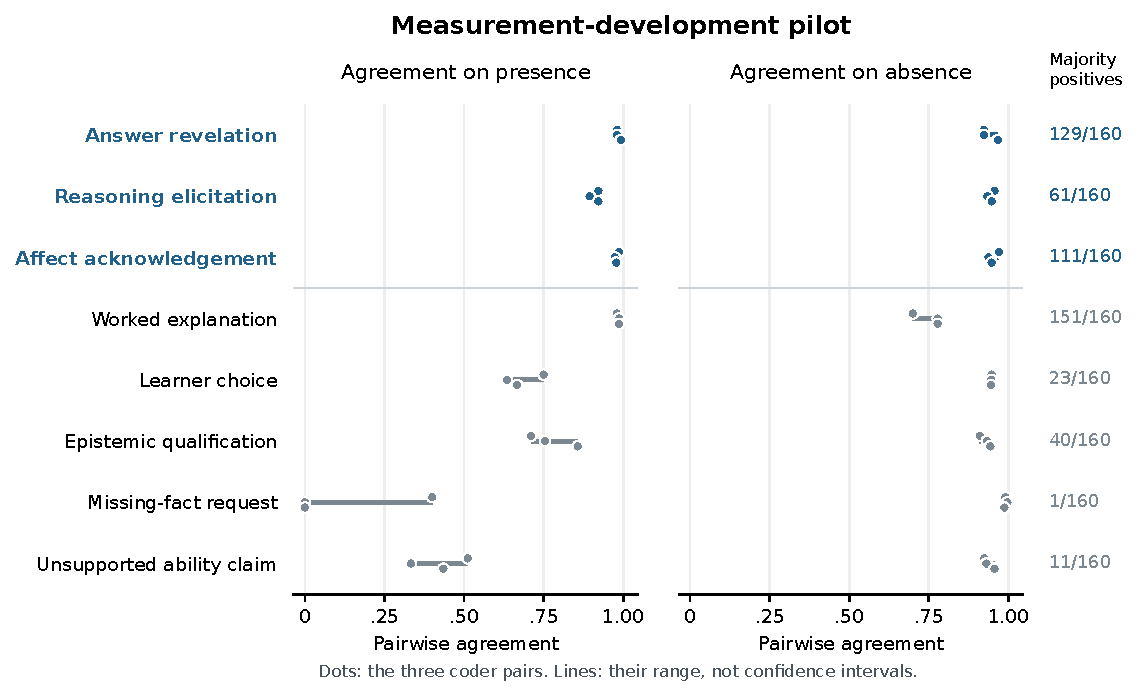
\includegraphics[width=\linewidth]{figures/measurement_pilot.pdf}
\caption{Completed measurement-development pilot: 160 tutor responses and 480
valid coder outputs. Each dot represents one of the three coder pairs; lines
span the observed pairs and are not confidence intervals. Blue labels identify
the three endpoints selected before formal generation. Agreement does not
establish semantic ground truth, and rare events require separate attention.}
\label{fig:pilot-measurement}
\end{figure}

Pilot model profiles suggest potentially useful defaults, but adding
student-state interactions does not consistently improve source-held-out
prediction over model-by-subject profiles during method development. These
exploratory observations motivated separate sources, within-domain replication,
and locked prospective comparisons. They are not substituted for the missing
confirmation outcomes.

\section{Limitations}

\paragraph{Scope of the construct.}
Educational personality denotes behavior observed in this educational setting.
We do not compare matched educational and non-educational interactions, so the
study cannot establish that a recurring tendency is unique to education.
The three primary events cover a small set of actions, can co-occur, and do not
constitute an independently validated latent trait structure. More predictable
behavior also need not be more helpful: answer revelation includes incorrect
conclusions, and elicitation can be appropriate or unhelpful depending on the
learner's needs. No learning outcome is measured.

\paragraph{Materials and transfer.}
The prospective sources are agent-authored English problems with scripted
student messages and supplied instructor references. They are not a probability
sample of classroom interactions. Four domains and two explicit student-cue
factors provide controlled comparisons, while leaving multilingual teaching,
extended dialogue, implicit learner cues, and advanced subject matter outside
the confirmation target. References equalize solution availability but cannot
eliminate differences in understanding or instruction following. The source
split prevents the specified problem families from crossing partitions; it
does not establish novelty relative to model pretraining.

\paragraph{Measurement and deployment.}
Automated content review and three answer coders avoid new human annotation,
but share possible model biases. Evidence-line checks verify location, and
coder-family exclusions test a particular dependence; neither guarantees
semantic validity. Rare or absent events require expression opportunities
before their absence can be interpreted. Five selected deployments are also
not a random sample of model families. Provider aliases and short-term repeated
requests cannot demonstrate long-term stability of weights or behavior. The
cross-stage sentinels mix generation variability, coding variability, and any
deployment drift, so they cannot identify those causes separately.

\paragraph{Inference and research history.}
There are 32 confirmation source groups, not thousands of
independent educational situations. Source intervals rely on an approximation
to variation across problems resembling this constructed bank. Small gains may
remain unresolved, and the conservative neutral-wording check cannot establish
population equivalence with sixteen sources. Conditional
prediction is limited to the selected student cues, feature blocks, and
regularized model class; a weak incremental gain does not disprove all
context-sensitive behavior. The archive analysis and pilot informed the study,
and some sensitivity and interpretation rules were fixed during training.
We disclose their timing and retain failed measurements. Local hashes and
execution timestamps support an inspectable sequence, but are not independent
third-party preregistration or tamper-proof timestamping.

\bibliographystyle{plainnat}
\bibliography{references}
\appendix
\section{Archive Scope and Historical Provenance}

The frozen archive census contains 1,028,822 raw records. Successful text
deduplication yields 899,025 model--benchmark--item--response records when
recorded input variants remain distinct, and 837,704 when variants are ignored
for text inventory only. Neither count estimates independent generation events.
Table~\ref{tab:archive-roles} classifies all 39 benchmark settings using a review
of current adapter contracts. Each assignment retains a source file, class,
line, hash, and interpretation note. Current contracts guide role interpretation
but do not establish the exact prompts used by every historical request.

\begin{table}[ht]
\centering\small
\begin{tabular}{lrr}
\toprule
Current task role & Settings & Records\\
\midrule
Evaluation of existing work & 7 & 354,308\\
Test or option answering & 10 & 306,307\\
Mixed educational assistance & 2 & 78,322\\
Tutor response & 9 & 68,799\\
Learner history or diagnosis & 2 & 42,997\\
Safety response & 2 & 13,974\\
Metacognitive problem solving & 3 & 11,188\\
Constrained question generation & 1 & 9,233\\
Assigned solution repair & 1 & 8,015\\
General instruction following & 1 & 3,782\\
Knowledge-structure reasoning & 1 & 2,100\\
\midrule
Total & 39 & 899,025\\
\bottomrule
\end{tabular}
\caption{Variant-preserving text inventory, not counts of independent tutoring
contexts or personality labels. Mixed educational assistance requires item-level
role separation; it is not automatically excluded from later research.}
\label{tab:archive-roles}
\end{table}

Evaluation and test/option outputs comprise 73.48\% of these records. For
example, the Pedagogy Benchmark requests pedagogical-knowledge multiple-choice
answers, while ASAP and SAS ask the candidate model to score student work.
MRBench and BEA judge settings likewise evaluate existing tutor text; that text
is not the candidate evaluator's own tutoring. Even among tutor settings,
instructions differ: TutorBench use cases request different actions, MMTutorBench
requires image-conditioned guidance in three prescribed sections, and LongTutor
explicitly requests scaffolding without the full answer.

A second pass verifies all 122 prediction files and corresponding summaries in
the nine tutor-response settings against the census hashes. Their 86,072 latest
successful file items reproduce 68,799 variant-preserving deduplicated records.
None of those file items contains the inspected fields for complete messages,
prompt text or input hashes, provider request identifiers, returned model names,
generation timestamps, or finish reasons. All contain usage metadata. Of the
122 summaries, 83 contain generation parameters and 114 contain a judge-prompt
hash; none contains the inspected generation-prompt hash fields. A judge-prompt
hash is not evidence of the tutor's generation prompt, and later scoring summaries
do not necessarily attest to the original generation parameters.

This is a field-coverage finding, not proof that provenance is unavailable in
external logs or original sources. Reconstructed historical inputs must be
identified as reconstructions. Consequently, the archive provides discovery and
confound audits, while the prospective study records the input, output, source,
version, and timing relationships needed for its own narrower confirmation.

\section{Detailed Methods and Protocol History}
\label{app:detailed-methods}

We use \emph{educational personality} operationally for recurring default
behavior and conditional response patterns of a deployed model in educational
interaction. Let $Y_{mqsar}^{(k)}$ denote whether model configuration $m$ expresses
behavior $k$ on source problem $q$, student state $s$, instruction arm $a$, and
independent request $r$. A default profile summarizes behavior under the
canonical tutor role over a specified distribution of educational inputs. A
conditional profile additionally represents how that behavior varies with
student state. We test both descriptions through predictions on separate source
problems. This operationalization does not require a fixed cross-context model
ranking, and it does not treat any identifiable linguistic signature as a
validated personality construct.

The unit $m$ is a deployment configuration, including its requested and returned
model names, provider, observation period, and generation settings. The five
prospective configurations request MiniMax-M3, MiniMax-M2.7, GLM-5.3,
DeepSeek-V4-Pro, and Doubao-Seed-2.0-Lite. In the measurement pilot, the request
alias GLM-5.2 returned GLM-5.3 throughout; those responses are identified by the
returned name and are not pooled with historical GLM-5.2 results. Provider model
names do not attest to immutable weights, so version and temporal uncertainty
remain limitations of deployment-level inference.




\subsection{Archive Exploration and Prospective Separation}

The archive audit distinguishes raw records from successful deduplicated
responses, and distinguishes tutors from solvers and evaluators. Repeated
questions and conversations can occur under different benchmark names and
prompt variants. Consequently, benchmark names and local item identifiers are
not sufficient independence units. Related source material must stay together
when estimating transfer. Analyses informed by previous archive results remain
exploratory; starting a new conversational context does not make them
prospective.

Across the 899,025 variant-preserving text records, a current-adapter role review
identifies 68,799 records in nine tutor-response settings; most other records
come from evaluation or test-answer tasks. Tutor-role membership does not itself
establish neutral prompts or equivalent historical requests. Appendix~A reports
the complete role inventory and a hash-verified inspection of the 122 tutor
prediction files, including their missing generation-provenance fields.

The controlled protocol uses 32 training questions in 30 conservative source
families and 32 confirmation questions in 32 separate source families. Each
partition has eight questions in each of mathematics, science, language, and
logic/data reasoning. Two training question pairs share an averaging or unit-
conversion family and remain grouped in internal validation. The four pilot
templates and their numerical substitutions are excluded. Confirmation tests
new sources within these four domains, rather than transfer to entirely new
academic domains or proof that a model has never encountered the underlying
concepts.

The questions, correct references, erroneous student attempts, and correct
unfinished work were authored by the research agent. Two model reviewers
checked 64 question packages before freezing, yielding 128 complete reviews.
All five Boolean content checks were positive in every review. Twenty-five
reviews nevertheless included issue text, mostly describing the deliberately
incorrect attempt or the deliberately unfinished work; these comments and their
agent adjudication are retained. This is content quality control without new
human annotation, not a human-gold validation claim.

\subsection{Crossed Educational Inputs}

Each main question has two student-work states, an erroneous attempt and correct
but unfinished work, crossed with two explicit affect statements, calm and
frustrated. These are four controlled input conditions. The work-state contrast
bundles correctness and progress; it does not isolate a pure progress or latent
student-ability effect. The affect statement is an input manipulation, not an
observation of a real learner's emotion.

All prospective main conditions provide the tutor with the same correct
instructor reference for that question, specifying that the student has not
seen it. This equalizes the availability of the solution but does not fully
control comprehension, attention, or instruction-following ability. Results
under this controlled reference condition are reported separately from the
historical archive.

The training stage uses the canonical tutor role on all 32 questions. The
confirmation stage first repeats this design on its 32 new questions. Within
each confirmation domain, four questions are selected by a fixed hash for four
additional role arms: two neutral paraphrases, an instruction to prioritize
student reasoning without revealing the final answer, and an instruction to
explain the solution and state the answer. Each selected question receives every
arm and student state. The neutral arms change only the role wording; the two
policy arms explicitly change the requested teaching behavior.

Every model--input cell receives two requests at temperature 0.7 with an
8,192-token output budget. The fixed design specifies 1,280 training responses,
1,280 canonical confirmation responses, and 2,560 additional intervention
responses. It also includes 160 secondary responses to paired complete/missing-
information probes on eight confirmation sources, plus 40 cross-stage responses
to four training-source sentinels. Sentinels and prompt variants do not increase
the count of independent confirmation sources. Request manifests, input hashes,
parameters, timestamps, and failure histories are recorded. Requests are
interleaved within shared provider concurrency limits rather than run as
separate model blocks.

\subsection{Observable Events and Measurement Development}

Three primary events are fixed from the measurement-development pilot.
\emph{Answer revelation} records an explicit final resolution, including an
incorrect resolution or a correct statement that information is insufficient.
It therefore measures disclosure, not correctness. \emph{Reasoning elicitation}
records an invitation for the student to perform unanswered reasoning, including
imperatives and indirect suggestions; rhetorical questions immediately answered
by the tutor do not qualify. \emph{Affect acknowledgement} records explicit
recognition of feeling or difficulty, excluding generic politeness and praise.
These are behavior endpoints, not three assumed independent personality factors.

Five secondary events cover worked explanation, learner choice, epistemic
qualification, requests for missing facts, and unsupported ability attribution.
All are retained regardless of their results. The pilot showed why a high
aggregate agreement rate is insufficient: requesting missing facts had only one
majority-coded positive example among 160 responses, while unsupported ability
attribution had weak positive agreement. Neither is promoted to a primary
endpoint based on subsequent confirmation results.

MiniMax-M3, DeepSeek-V4-Pro, and GLM-5.3 each code every visible tutor response.
Coders receive the student conversation, the reference target, and the answer
with original line identifiers. They do not receive the generating model name,
system-role assignment, repeat number, or partition label. Natural output style
can still reveal identity. Positive codes must reference existing nonempty
source lines; negative codes have no references. Valid references establish
traceability, not semantic truth. We use majority labels when all three coders
are structurally valid, and retain individual and leave-one-coder analyses,
including fractional means for two-coder ties.

The initial exact-quotation protocol failed on naturally formatted answers,
which motivated line references during measurement development. Original
failures remain archived. The finalized pilot has 480 valid codes for 160
unchanged tutor responses after two structure/completion failures were retried
under identical inputs. Formal structure failures are likewise recorded and
retried without selecting by event label or coder agreement.
A training coding interruption was recovered using saved valid outputs and
the existing two-pass repair allowance. This yielded 3,839 of 3,840 valid codes.
One GLM coding request repeatedly exhausted its 16,384-token completion budget
without visible output. Before forecast locking or confirmation generation, a
disclosed amendment allowed this single missing code a 32,768-token ceiling
and at most two attempts, keeping its model, input, rubric, and temperature
fixed. It completed on the first attempt using 3,511 completion tokens; this
does not identify the cause of the preceding failures. The original and
expanded-budget groups were validated separately before their disjoint codes
were combined. All 1,280 training answers consequently have three valid codes.
The interrupted run, failed attempts, and amendment receipt are retained; the
single expanded-budget code is an explicit deviation from the original
uniform-budget protocol.

\subsection{Prediction Before Confirmation Generation}

For each behavior, four nested logistic predictors model the probability of its
occurrence: a subject-by-student-state baseline; that baseline plus model
identity; an additional model-by-subject block; and an additional
model-by-student-state block. New feature blocks are orthogonalized against
existing blocks using training data and standardized under source-equal
weights. This prevents duplicate main-effect encodings from changing their
ridge penalty when interactions are introduced. The intercept is unpenalized.
The penalty is selected from $\{0.1,1,10,100\}$ by source-grouped training-only
validation. Constant training outcomes use the same smoothed constant across
all four predictors.

The fitted models, tuning choices, input hashes, and confirmation probabilities
are saved before any confirmation tutor response is generated. The generation
runner checks this prediction lock. No confirmation label, answer length, or
same-item cross-model score enters a primary predictor. A secondary competing
forecast uses only training-source profiles of log word count and marked-line
fraction, recomputing those profiles within training validation. Such style
competition is descriptive: teaching policy may itself influence length and
formatting, so it is not a causal adjustment for style.

For each of the three primary events, the two primary comparisons are the Brier
improvement from a default model profile over the situation baseline and from a
student-state profile over the model-by-subject baseline. We average losses
within source and then equally across the 32 confirmation sources. The six
one-sided paired source-level tests use Holm correction. We report absolute
Brier losses, source-bootstrap intervals, and all comparison signs. These
intervals condition on the fitted training profiles and a source-sampling
approximation; they do not describe uncertainty over all models or all
educational contexts.

\subsection{Repetition and Prompt Plasticity}

Repetition analyses report positive, negative, and total event agreement and
profile correspondence, retaining source clustering. Constant behavior can
produce perfect repeat agreement and is reported as such. On the 16 fully
crossed intervention sources, we estimate each model's event-rate difference
between an alternative role and the canonical role. We report average shifts
alongside model and student-state heterogeneity.

For neutral wording, the fixed equivalence reference is $\pm0.10$ in event
probability. We retain the nominal Bonferroni paired-$t$ intervals across the
30 model--event--neutral-arm comparisons. A nonsignificant difference does not
establish equivalence, and constant source differences receive a degeneracy
flag. Further synthetic diagnostics during training show undercoverage in a
sparse boundary case even with nonzero source variance. Before confirmation
generation, we therefore additionally require a bounded-source interval to
support any population-equivalence statement. Scaling Hoeffding's bound to
source differences in $[-1,1]$ and allocating error across both tails and all
30 comparisons gives half-width
$\sqrt{2\log(2\cdot30/0.05)/n}$ \citep{hoeffding1963}. At $n=16$ this is
approximately $0.941$, too wide to support the chosen tolerance. This
conservative sensitivity still assumes independent source observations and
does not make the authored bank representative. We can describe observed
neutral shifts and nominal intervals, while withholding population equivalence.
These disclosed interpretation additions preserve the frozen numerical output
and the six primary prediction tests. The
explicit ASK and EXPLAIN arms quantify policy displacement rather than better
teaching. Finally, answer revelation and reasoning elicitation are analyzed
jointly as four possible combinations. Their evidence lines do not identify
which action occurred first, and we do not infer action order from them.

\subsection{Sensitivity Analyses and Their Timing}

During training coding, after measurement development but before confirmation
responses exist, we additionally fix eight alternative coding panels: the
three-coder mean, each individual coder, each two-coder mean, and the mean after
excluding the generator's model family. For each panel, forecasts are refitted
using its training labels and locked before confirmation generation. They are
evaluated against the corresponding confirmation labels; two-coder ties remain
0.5. This checks dependence on coding choices but cannot remove biases shared
by all coders or supply an external ground truth.

Five further forecast sets each remove one generator configuration from both
training and the confirmation target, refitting the baselines and tuning within
the retained training data. This checks dependence on a single configuration;
it changes the target model mixture and does not test prediction of an unseen
model. Neither sensitivity family replaces the six primary comparisons.

We also resample the 30 training source families 200 times, preserving the
multiplicity of repeated source draws. We retain the selected regularization
relative to total loss weight, without repeating hyperparameter selection, and
recompute training-style profiles in each resample. The resulting gain quantiles
describe training-source sensitivity conditional on the confirmation material
and selected regularization. They are separate from the primary confirmation-
source intervals. These extensions were specified before confirmation outputs,
not preregistered before the entire research project began.

\subsection{Mathematics and Content-Error Sensitivity}

The protocol also requires a mathematics subset and a check of dependence on
obvious content errors. Its implementation is fixed during training coding,
before confirmation generation. We evaluate the existing forecasts on all eight
mathematics sources, covering 320 canonical responses, without refitting.
Separately, MiniMax-M3 and DeepSeek-V4-Pro review all 1,280 canonical responses
for checkable content errors using the student input, reference, and original
answer lines. They distinguish a clear error, no clear error identified, and
uncertainty. Withholding a solution, asking a question, or correctly quoting
and correcting an error is not itself an error. Positive error judgments
require a category and source-line evidence.

Twelve agent-authored controls accompany the responses, giving 2,584 planned
secondary review requests. Each reviewer must match at least five of six
controls in each of the clear-error and no-clear-error classes to meet the
limited diagnostic rule. If either reviewer fails, screened results remain
measurement-limited diagnostics. These controls do not establish correctness
on natural responses, even when the rule is met.

We retain the full primary results and report three additional screens:
excluding unanimously identified errors; excluding errors identified by either
reviewer; and excluding either errors or uncertainty. A flagged response
removes its entire five-model source--student-state--repeat slot so that model
comparisons remain paired. We report retained coverage and source-equal losses
with descriptive source intervals, without new hypothesis tests. These screens
condition on generated responses and change the target distribution; they are
not causal controls for ability. The content review covers the canonical panel,
not all prompt-intervention responses.

\end{document}
